\chapter{Implementation}
\label{chap:ch3}

\par The backend of Doclane is written in Go, and the frontend is built with Next.js. Go was chosen because it is fast, has a large standard library, and handles errors in a way that makes bugs easier to track. Next.js was chosen because Doclane is a dynamic application that makes many requests to the backend, and server-side rendering helps keep loading times short.

\begin{center}
    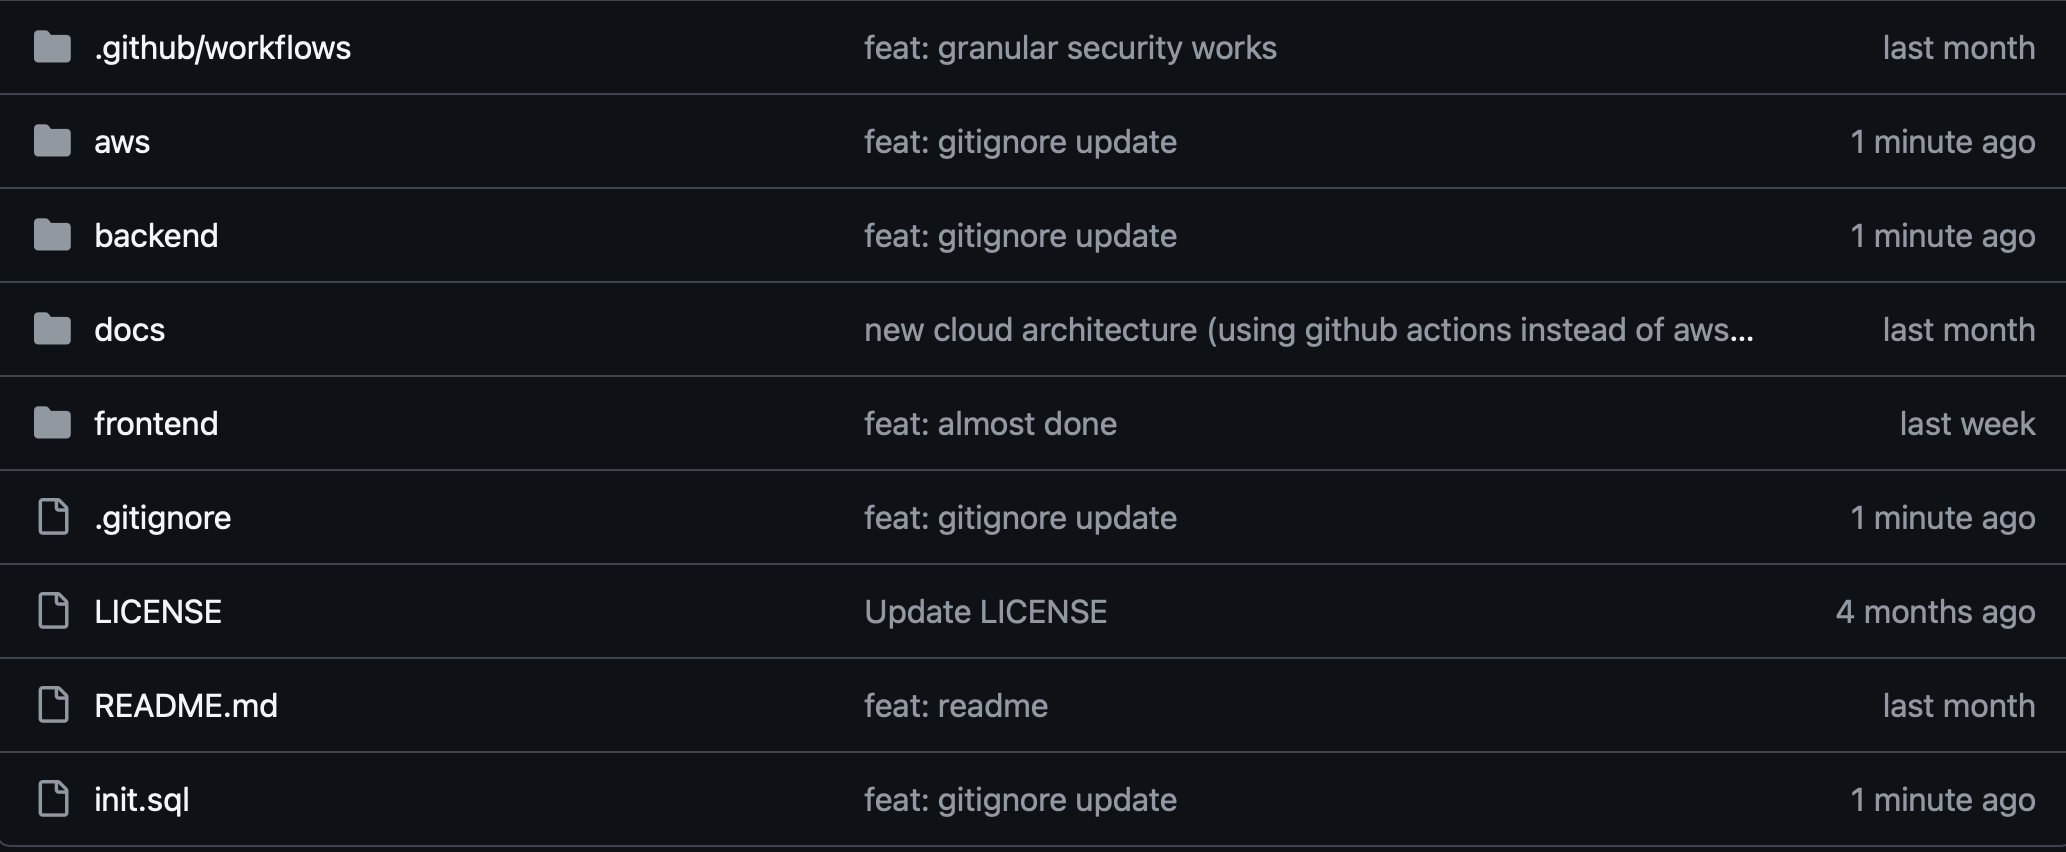
\includegraphics[width=0.8\textwidth]{figures/folder-structure.png}
    \captionsetup{type=figure}
    \captionof{figure}{Overview of Doclane's folder structure.}
\end{center}

\section{Backend}

\subsection{Go}

\par Go is a statically typed, compiled programming language. It has a simple syntax and a standard library that covers most common needs. It is also fast to write and produces efficient binaries.

\subsection{Layers}

\par The backend code is split into four layers:

\begin{itemize}
    \item Handler layer: handles incoming HTTP requests and extracts the needed information from them, such as JWT claims, resource IDs, or uploaded files.
    \item Service layer: contains the business logic and validations. For example, it checks whether a user has the right role to perform an action. A user cannot view the files of a request unless they are an admin or they belong to the department that manages that request.
    \item Repository layer: executes queries on the database. It trusts everything passed to it, since all validation happens in the service layer. Transactions are used when multiple database operations need to succeed together for an action to be considered complete.
    \item Model layer: holds the data structures used across the application, such as users, requests, templates, invitation codes, and comments. DTOs (Data Transfer Objects) are used in some cases to enrich data from the database. For example, when retrieving a request, the DTO also includes the requester's name and email, not just their ID.
\end{itemize}

\subsection{Authentication}

\par Authentication is handled using JWTs (JSON Web Tokens) issued by AWS Cognito. A JWT is a stateless token that contains information about the user such as their ID, role, department, and name. The information inside the token is readable by anyone, but it cannot be changed without the signature becoming invalid. The backend rejects any token with an invalid signature.

\par The token is stored in an HTTP-only cookie. This means JavaScript running in the browser cannot access it, which protects against XSS (Cross-Site Scripting) attacks. More details about Cognito and how it is configured are in chapter 4.

\subsection{API Response}

\par Every response from the API follows the same structure. This makes it easier for the frontend to handle responses in a consistent way. Every response contains:

\begin{itemize}
    \item \textbf{success} - a boolean that says whether the request worked or not.
    \item \textbf{message} - optional, a short description of what happened.
    \item \textbf{error} - optional, an error message present when success is false.
    \item \textbf{data} - optional, contains any data returned by the request.
\end{itemize}

\begin{center}
    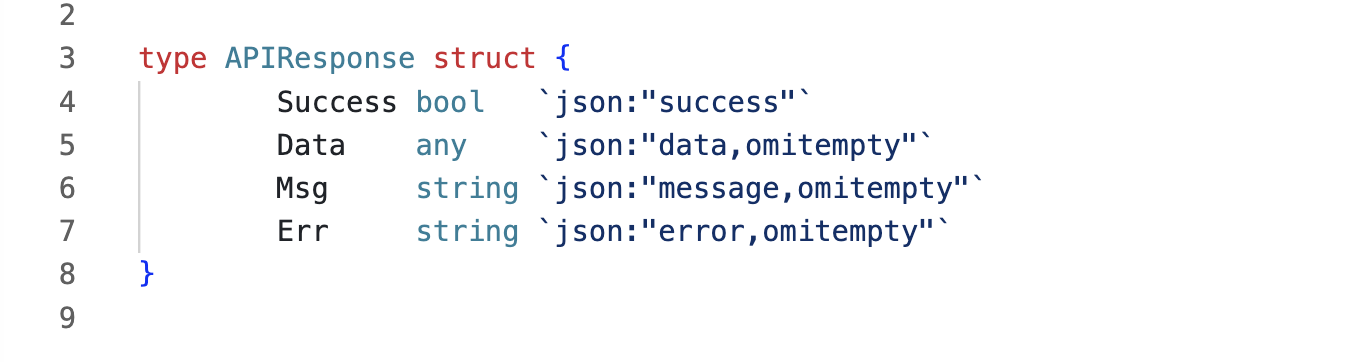
\includegraphics[width=0.8\textwidth]{figures/api-response.png}
    \captionsetup{type=figure}
    \captionof{figure}{API Response struct.}
\end{center}

\subsection{Custom Errors}

\par Custom error types are defined and used across the backend. This gives a unified way to handle errors and makes the code easier to read.

\subsection{Configuration}

\par There is a single configuration file that acts as the main setup for the application. It is where all service and repository instances are created and exported. If a repository implementation needs to be changed, only this file needs to be updated. Everything else continues to work without changes.

\subsection{Middleware}

\par Most routes in the application are protected by middleware. The middleware checks that every incoming request has a valid JWT token before it reaches the handler. Requests with missing or invalid tokens are rejected early.

\par There are two middleware checks in Doclane. The first checks that the token is valid and was signed correctly by Cognito. The second checks that the user account is active.

\subsection{File Storage}

\par Uploaded files are stored in S3, which is a file storage service from AWS. The file storage logic is separated from the rest of the application so the app does not depend on it directly. All file access is done through presigned URLs, which are temporary links that give access to a specific file for a limited time. More details about S3 and how it is set up are in chapter 4.

\subsection{Routing}

\par Backend routing is done using the Chi library, which is a third party Go package. Although Go's standard library handles many things well, HTTP routing is an area where external help is useful. Chi makes it easy to organize routes in a clear and readable way.

\begin{center}
    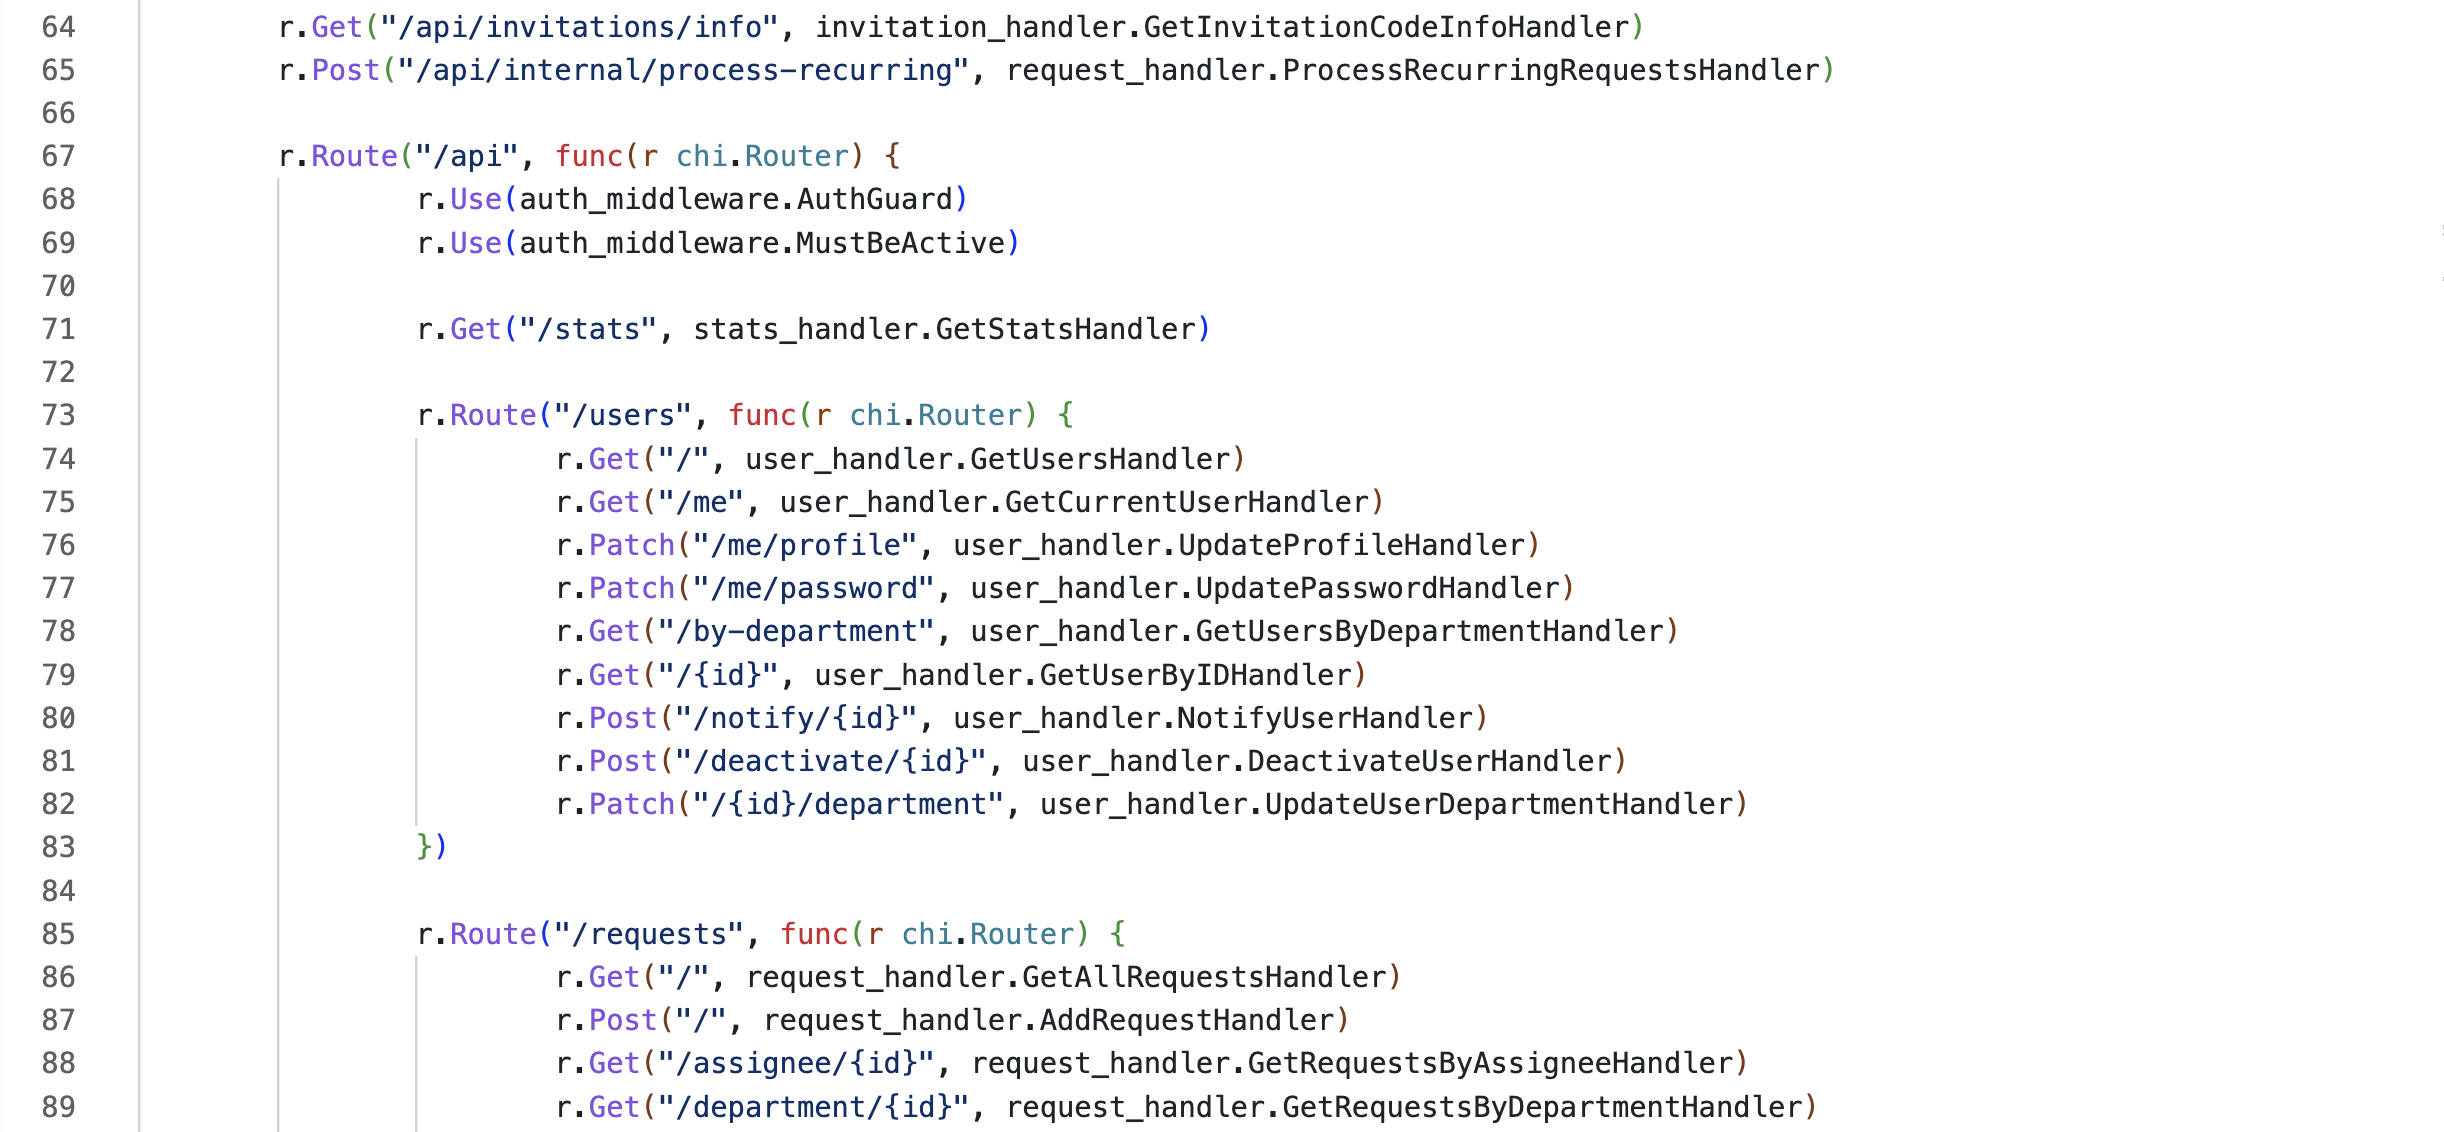
\includegraphics[width=0.8\textwidth]{figures/implementation/backend/chi-routes.png}
    \captionsetup{type=figure}
    \captionof{figure}{Routing for the backend.}
\end{center}

\section{Database}

\par PostgreSQL was chosen as the database engine. It is one of the most widely used relational databases and it fits the needs of Doclane well since the data has clear relationships between tables.

\begin{center}
    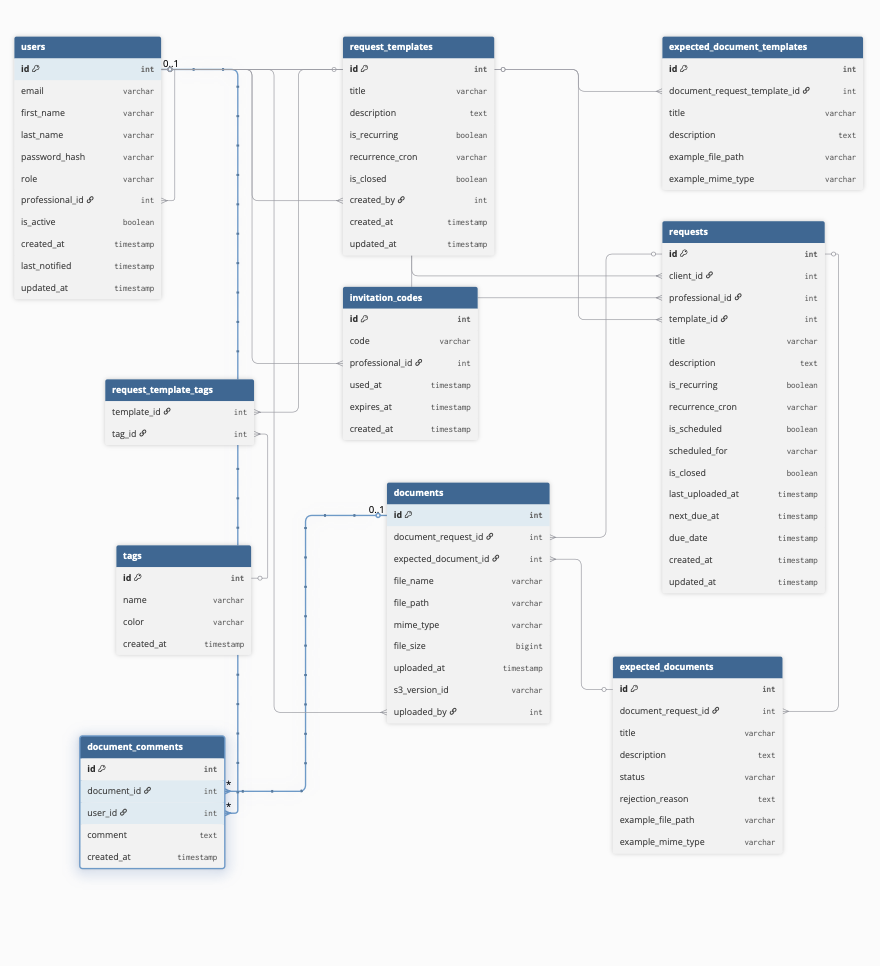
\includegraphics[width=0.8\textwidth]{figures/implementation/backend/database-diagram.png}
    \captionsetup{type=figure}
    \captionof{figure}{Database schema overview.}
\end{center}

\section{Frontend}

\par The frontend is built with Next.js, which is an open-source web framework built on top of React. It supports server-side rendering, which means pages can be prepared on the server before being sent to the browser.

\par Next.js was chosen because Doclane makes many requests to the backend on almost every page. If a client-side only framework like plain React was used, users would spend a lot of time on loading screens. With Next.js, data is fetched on the server before the page is shown, so the experience is faster.

\par Frontend code is split into small reusable components so that the same piece of UI does not need to be written more than once. This follows the DRY (Don't Repeat Yourself) principle, which is also applied in the backend but is most visible in the frontend.